% Capítulo de la tesis: antecedentes del caso (antes en el marco teórico) y análisis de los datos (antes en la metodología).
\chapter{Datos}
\label{sec:datos}

Este capítulo presenta los datos con que se contrastan las hipótesis. La Sección~\ref{sec:antecedentes} describe las economías y los episodios de estrés del período. Las Secciones~\ref{sec:panel},~\ref{sec:embi} y~\ref{sec:controles} detallan el panel, la variable dependiente y los controles. La Sección~\ref{sec:descriptiva} resume la muestra de estimación, y la Sección~\ref{sec:trayectorias} muestra cómo se mueven en el tiempo la fragilidad, el riesgo de cola y el spread. La construcción de las dos métricas está en las Secciones~\ref{sec:jloss} y~\ref{sec:gar}.

\section{Antecedentes del caso}
\label{sec:antecedentes}

\textbf{Las economías.} El estudio cubre trece economías emergentes: Brasil, Chile, Colombia, México y Perú en América Latina; China, Filipinas, India, Indonesia y Malasia en Asia; Polonia y Turquía en Europa emergente, y Sudáfrica. Todas tienen deuda soberana en dólares en el EMBI de J.P.\ Morgan, el indicador de spread que usan \citet{Chari2024b} y esta tesis. Difieren en quién tiene su deuda: la participación de no residentes va, en promedio, de un 64\% en Perú a un 3\% en China (Sección~\ref{sec:participacion-extranjera}). Difieren también en la fragilidad de su banca. Malasia, Perú, Indonesia y Sudáfrica tienen una fragilidad media cercana al piso de la métrica; Turquía, India y China, la más alta (Sección~\ref{sec:descriptiva}).

\textbf{Los episodios de estrés.} El período 2004--2026 tiene tres episodios de estrés que el análisis trata por separado, porque el respaldo oficial que recibieron las economías emergentes fue distinto. La crisis financiera global (2008Q4--2009Q4) y la pandemia (2020Q1--2021Q4) tuvieron respaldo a escala global: líneas de \textit{swap} de la Reserva Federal (en el panel, solo para Brasil y México), financiamiento del FMI, incluidas sus Líneas de Crédito Flexible, y compras de activos. El estrés emergente de 2015Q3--2016Q1 no tuvo nada comparable. Hubo además dos ventas de activos emergentes más breves: el \textit{taper tantrum} de 2013 y la venta masiva de 2018. La Sección~\ref{sec:est-crisis} formaliza la distinción y la Sección~\ref{sec:respaldo-pais} mide el respaldo por país y fecha.

\textbf{Cuándo coinciden los tres.} La fragilidad bancaria, el riesgo de cola del crecimiento y el spread se mueven juntos en episodios puntuales: Brasil, Colombia, México y Polonia en 2008--09 y en 2020; Brasil también en 2015--16, y Turquía entre 2018 y 2021 (Figura~\ref{fig:series}). Fuera de esos episodios, las tres series son moderadas y estables. Como la coincidencia se concentra en pocos episodios, la simultaneidad de los dos riesgos se documenta con cuidado (Sección~\ref{sec:simultaneidad}), y el análisis declara qué se puede afirmar con trece países.

\section{El panel}
\label{sec:panel}

El panel es trimestral y reúne las economías emergentes que tienen $JLoss$, $GaR$ y EMBI. Los insumos micro de $JLoss$ vienen de Bloomberg; los componentes reales del FCI (IPC, PIB, índice accionario, tipo de cambio real y rendimiento a diez años), de las estadísticas nacionales; el VIX, de Bloomberg. El Anexo~\ref{chap:anexoA} tabula la procedencia de cada serie.

Una economía entra al panel si tiene $JLoss$, y solo se excluye cuando $JLoss$ no es una medida válida para el país. Corea del Sur queda fuera porque el valor de mercado de su banca está siempre cerca del 4\% del punto de incumplimiento (el \textit{Korea discount}), y el modelo de Merton lo lee como un incumplimiento inminente. Bulgaria y Hungría quedan fuera porque cotizan solo uno y dos de sus bancos, respectivamente, y la métrica no representaría un sistema bancario.

La muestra de estimación de la especificación principal exige el EMBI del trimestre y $JLoss$ y $GaR$ del trimestre anterior, sin huecos. Son trece economías y 765 observaciones país-trimestre (2004Q2--2026Q2). La Figura~\ref{fig:cobertura} muestra la cobertura de cada una.

\begin{figure}[htbp]
\centering
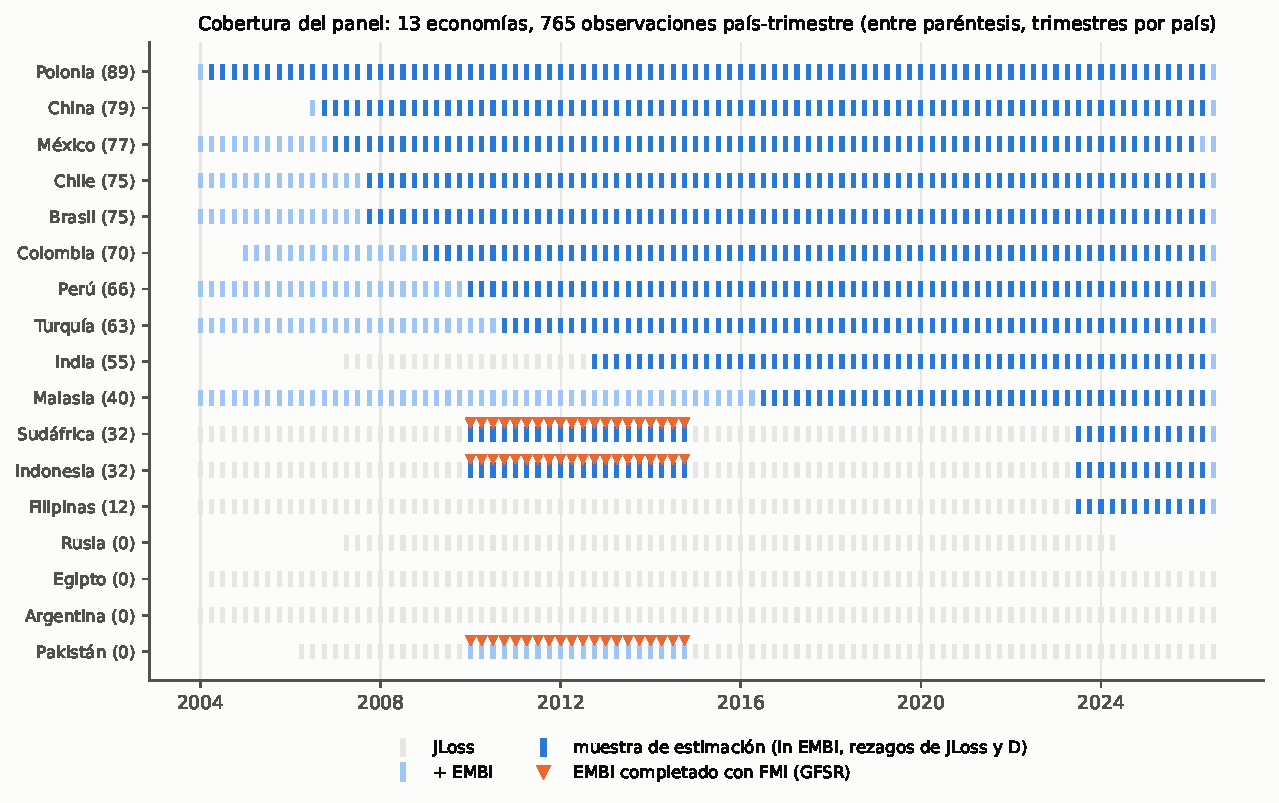
\includegraphics[width=\textwidth]{fig_cobertura_embiext.pdf}
\caption[Cobertura del panel]{Cobertura del panel, por país. Gris: trimestres con $JLoss$. Celeste: además con EMBI. Azul: muestra de estimación de la especificación principal. Triángulos: trimestres en que el EMBI proviene de la serie del FMI (GFSR). Entre paréntesis, trimestres de estimación por país.}
\label{fig:cobertura}
\end{figure}

Como se ve en la figura, la historia disponible es desigual. Diez economías aportan una historia larga, de entre 40 y 89 trimestres, limitada por el inicio del $GaR$ o del EMBI: Brasil, Chile, China, Colombia, India, Malasia, México, Perú, Polonia y Turquía. Filipinas aporta 12 trimestres; Indonesia y Sudáfrica, 32 cada una. Egipto, Pakistán y Rusia tienen $JLoss$ pero ninguna observación, porque les falta el EMBI, el $GaR$ o el solapamiento entre ambos.

Argentina sí completa las tres series. Su $GaR$, sin embargo, se estimó con un índice de condiciones financieras sin el bloque de tasas y con una ventana de estandarización más corta, por la breve historia de su IPC oficial. Por esa desviación queda fuera de la muestra principal y entra como ejercicio de robustez (34 observaciones, spread de 2017Q3 a 2025Q4; Sección~\ref{sec:robustez-argentina}).

\section{Variable dependiente: el EMBI}
\label{sec:embi}

El spread soberano se mide con el EMBI Global Diversified de J.P.\ Morgan, como en \citet{Chari2024b}. El valor trimestral del panel es el \emph{promedio} de los días del trimestre, no su cierre, y eso importa para el orden temporal. $JLoss_{t-1}$ usa la capitalización bursátil del cierre de $t-1$, así que el cambio del spread promedio entre $t-1$ y $t$ contiene movimientos ocurridos dentro de $t-1$. Por eso se construyen también, desde la serie diaria, el spread de cierre (los últimos cinco días hábiles del trimestre) y el promedio del primer mes, que usa la Sección~\ref{sec:estacionariedad}.

La serie de J.P.\ Morgan disponible para Indonesia y Sudáfrica empieza en 2023Q3. Para ellas, el período 2010Q1--2014Q4 se completa con la serie trimestral de spreads soberanos del FMI (\textit{Global Financial Stability Report}), que trae un solo valor por trimestre. El empalme se valida en las economías que tienen ambas series: en 80 trimestres de solapamiento (China, Hungría, Polonia y Turquía) correlacionan 0,94, con una razón mediana de 1,02, y por eso se usan sin reescalar. La serie del FMI solo llena trimestres sin dato de J.P.\ Morgan, y la Sección~\ref{sec:robustez} verifica que excluir esos 40 trimestres no cambia los resultados.

\section{Controles}
\label{sec:controles}

Los controles domésticos son la deuda del gobierno general/PIB y el balance fiscal/PIB (FMI), las reservas/PIB y la cuenta corriente/PIB (Banco Mundial), la inflación interanual y el tipo de cambio real efectivo. Son series anuales interpoladas a frecuencia trimestral y cubren 649 de las 765 observaciones de la muestra principal.

\section{Estadística descriptiva}
\label{sec:descriptiva}

La Tabla~\ref{tab:descriptivos} resume la muestra de estimación. El spread promedia 198 puntos básicos, con una mediana de 177 y un máximo de 661. $JLoss_{t-1}$ tiene una media de 4,65 y una mediana de 2,67: la fragilidad sistémica se concentra en pocos episodios y países.

\input{\tablasdir/tabla_descriptivos_embiext}

La métrica de fragilidad tiene además un piso. Se amontona en $2{,}16$, el techo de la malla de pérdidas del motor en sus unidades ($0{,}048\times0{,}45\times100$), y el 23,7\% de las observaciones está a menos de un 2\% de ese valor. Turquía (9,6), India (8,4) y China (6,8) están en el extremo superior (Tabla~\ref{tab:mediaspais}); Malasia, Perú, Indonesia y Sudáfrica tienen una fragilidad media cercana al piso. En el piso la variable no informa, y por eso las magnitudes se leen por desviación estándar dentro del país, no por unidad ni por cambio porcentual de $JLoss$ (Sección~\ref{sec:magnitud}).

$D_{t-1}$ promedia $-1{,}5$ puntos porcentuales ---en el trimestre típico, el cuantil 5\% del crecimiento es positivo---, con una cola que llega a $+17{,}7$ en los episodios de estrés. Su desviación estándar es de 3,7 puntos en el panel completo y de 3,1 dentro del país, la unidad que se usa en adelante.

La descomposición de la varianza (Tabla~\ref{tab:varianza}) importa para identificar con efectos fijos de país. El 82\% de la desviación de $\ln JLoss_{t-1}$, el 84\% de la de $D_{t-1}$ y el 67\% de la de $\ln$ EMBI es variación \textit{within}: dentro de cada país, a lo largo del tiempo. Deuda/PIB y reservas/PIB, en cambio, son sobre todo transversales (53\% y 52\% \textit{within}).

La Figura~\ref{fig:distribuciones} muestra las distribuciones univariadas. El logaritmo reduce la asimetría de $JLoss$ de 2,79 a 1,34 y la del EMBI de 1,20 a $-0{,}74$.

\begin{figure}[htbp]
\centering
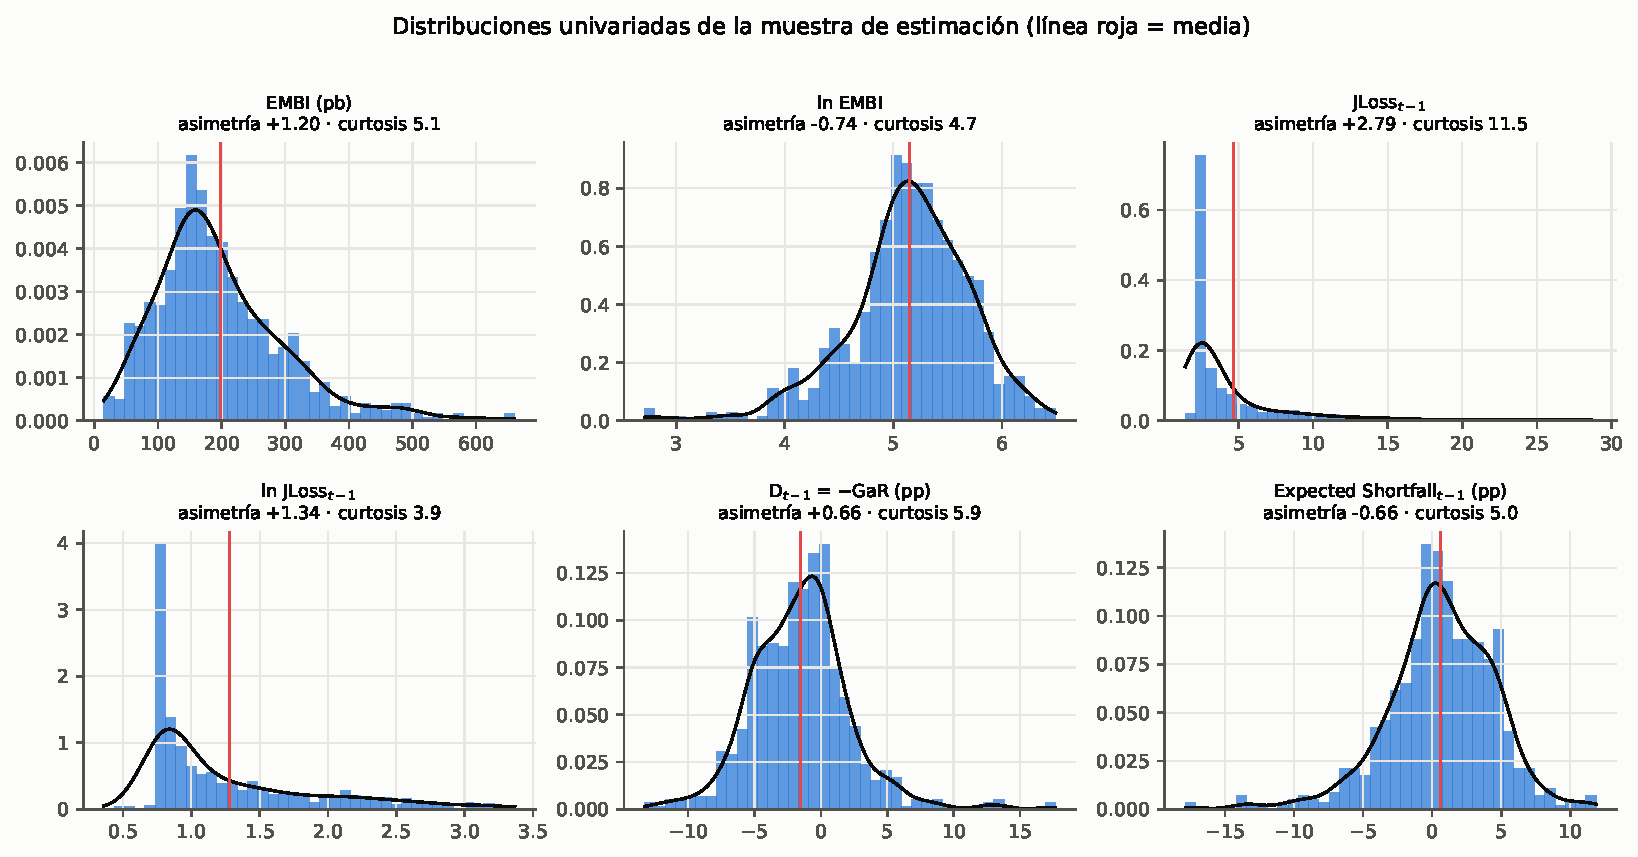
\includegraphics[width=\textwidth]{fig_distribuciones_embiext.pdf}
\caption[Distribuciones univariadas]{Distribuciones univariadas de la muestra de estimación (línea roja: media). La transformación logarítmica comprime la asimetría del spread y de $JLoss$.}
\label{fig:distribuciones}
\end{figure}

La Figura~\ref{fig:correlaciones} presenta la matriz de correlaciones. $D$ y el \textit{Expected Shortfall} correlacionan $-0{,}98$: son la misma información sobre la cola. $\ln JLoss_{t-1}$ correlaciona $-0{,}48$ con el balance fiscal, $+0{,}41$ con la inflación y $+0{,}31$ con la deuda, lo que anticipa por qué los controles la absorben en la Sección~\ref{sec:bateria}. La correlación lineal entre $\ln JLoss_{t-1}$ y $D_{t-1}$ es moderada (0,16 en el panel; 0,26 descontados los efectos fijos de país y de tiempo), pero sus valores altos coinciden mucho más a menudo de lo que esa correlación sugiere (Sección~\ref{sec:simultaneidad}).

\begin{figure}[htbp]
\centering
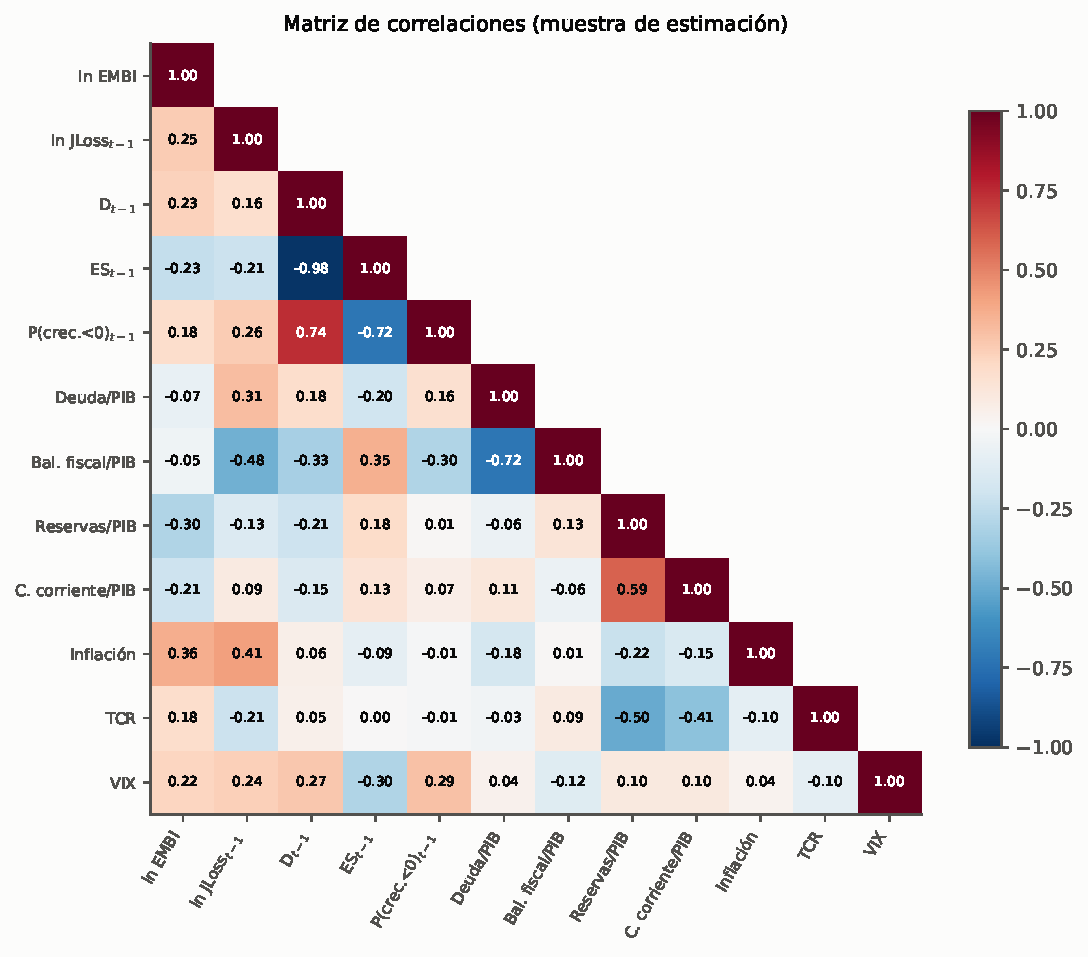
\includegraphics[width=0.82\textwidth]{fig_correlaciones_embiext.pdf}
\caption[Matriz de correlaciones]{Matriz de correlaciones de la muestra de estimación. $JLoss$, $D$, ES y $P(\text{crec.}<0)$ rezagados un trimestre; controles contemporáneos.}
\label{fig:correlaciones}
\end{figure}

\section{Trayectorias y co-movimiento}
\label{sec:trayectorias}

Las Figuras~\ref{fig:jlosspaises} y~\ref{fig:garpaises} trazan $JLoss$ y $D$ por país. Las dos series son moderadas y estables en los períodos normales y se disparan en episodios puntuales, no siempre simultáneos entre países; esa es la variación que identifica la interacción.

\begin{figure}[htbp]
\centering
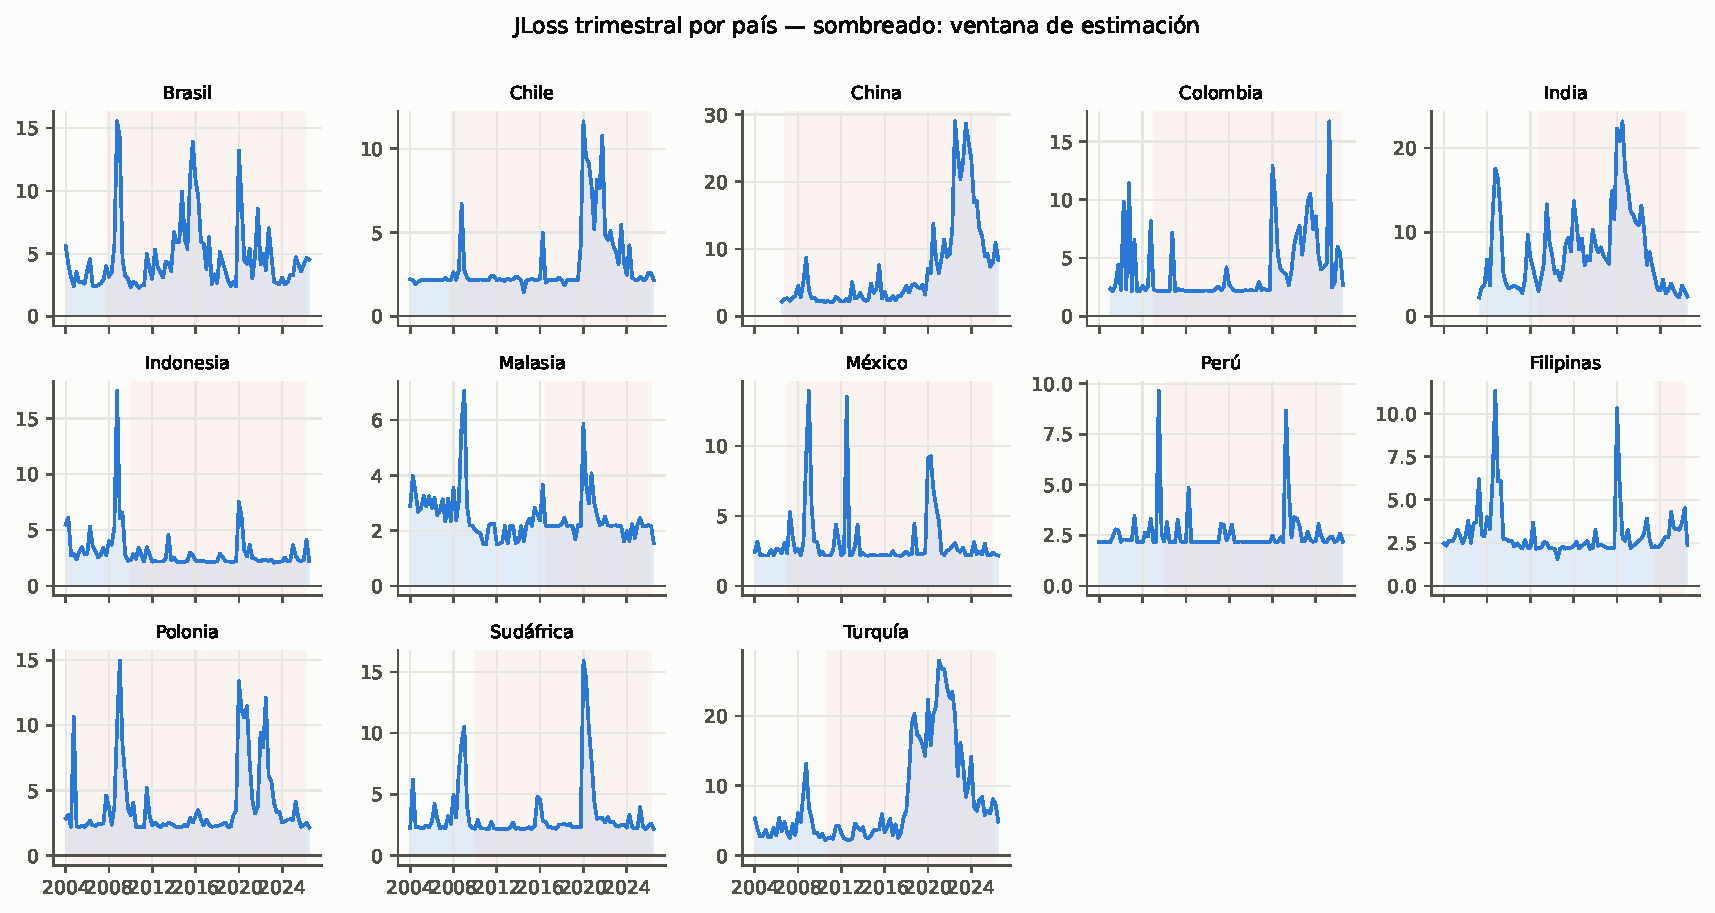
\includegraphics[width=\textwidth]{fig_jloss_paises_embiext.pdf}
\caption[JLoss por país]{$JLoss$ trimestral por país (motor de punto de silla sobre datos Bloomberg). Sombreado: ventana de estimación.}
\label{fig:jlosspaises}
\end{figure}

\begin{figure}[htbp]
\centering
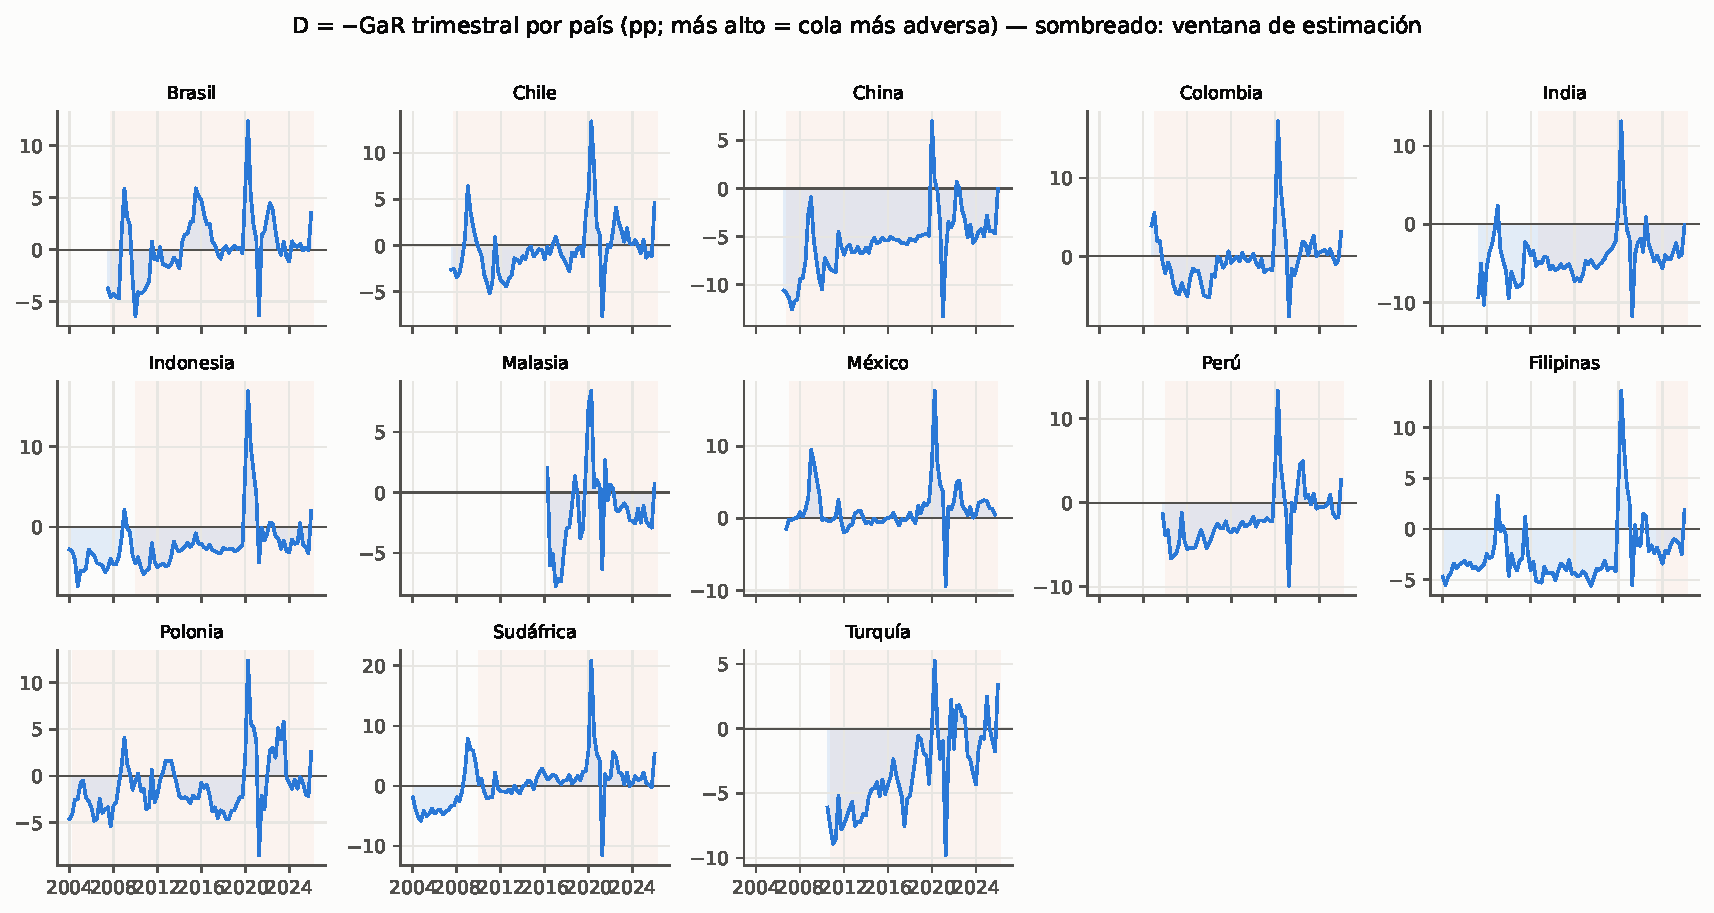
\includegraphics[width=\textwidth]{fig_gar_paises_embiext.pdf}
\caption[Riesgo de cola por país]{$D=-GaR$ trimestral por país (puntos porcentuales; más alto indica una cola más adversa). Sombreado: ventana de estimación.}
\label{fig:garpaises}
\end{figure}

La Figura~\ref{fig:series} superpone, por país, la fragilidad, el riesgo de cola y el spread, con el vector de crisis sombreado. En Brasil, Colombia, México y Polonia los tres se mueven juntos en 2008--09 y en 2020; en Brasil también en 2015--16, y en Turquía entre 2018 y 2021.

\begin{figure}[htbp]
\centering
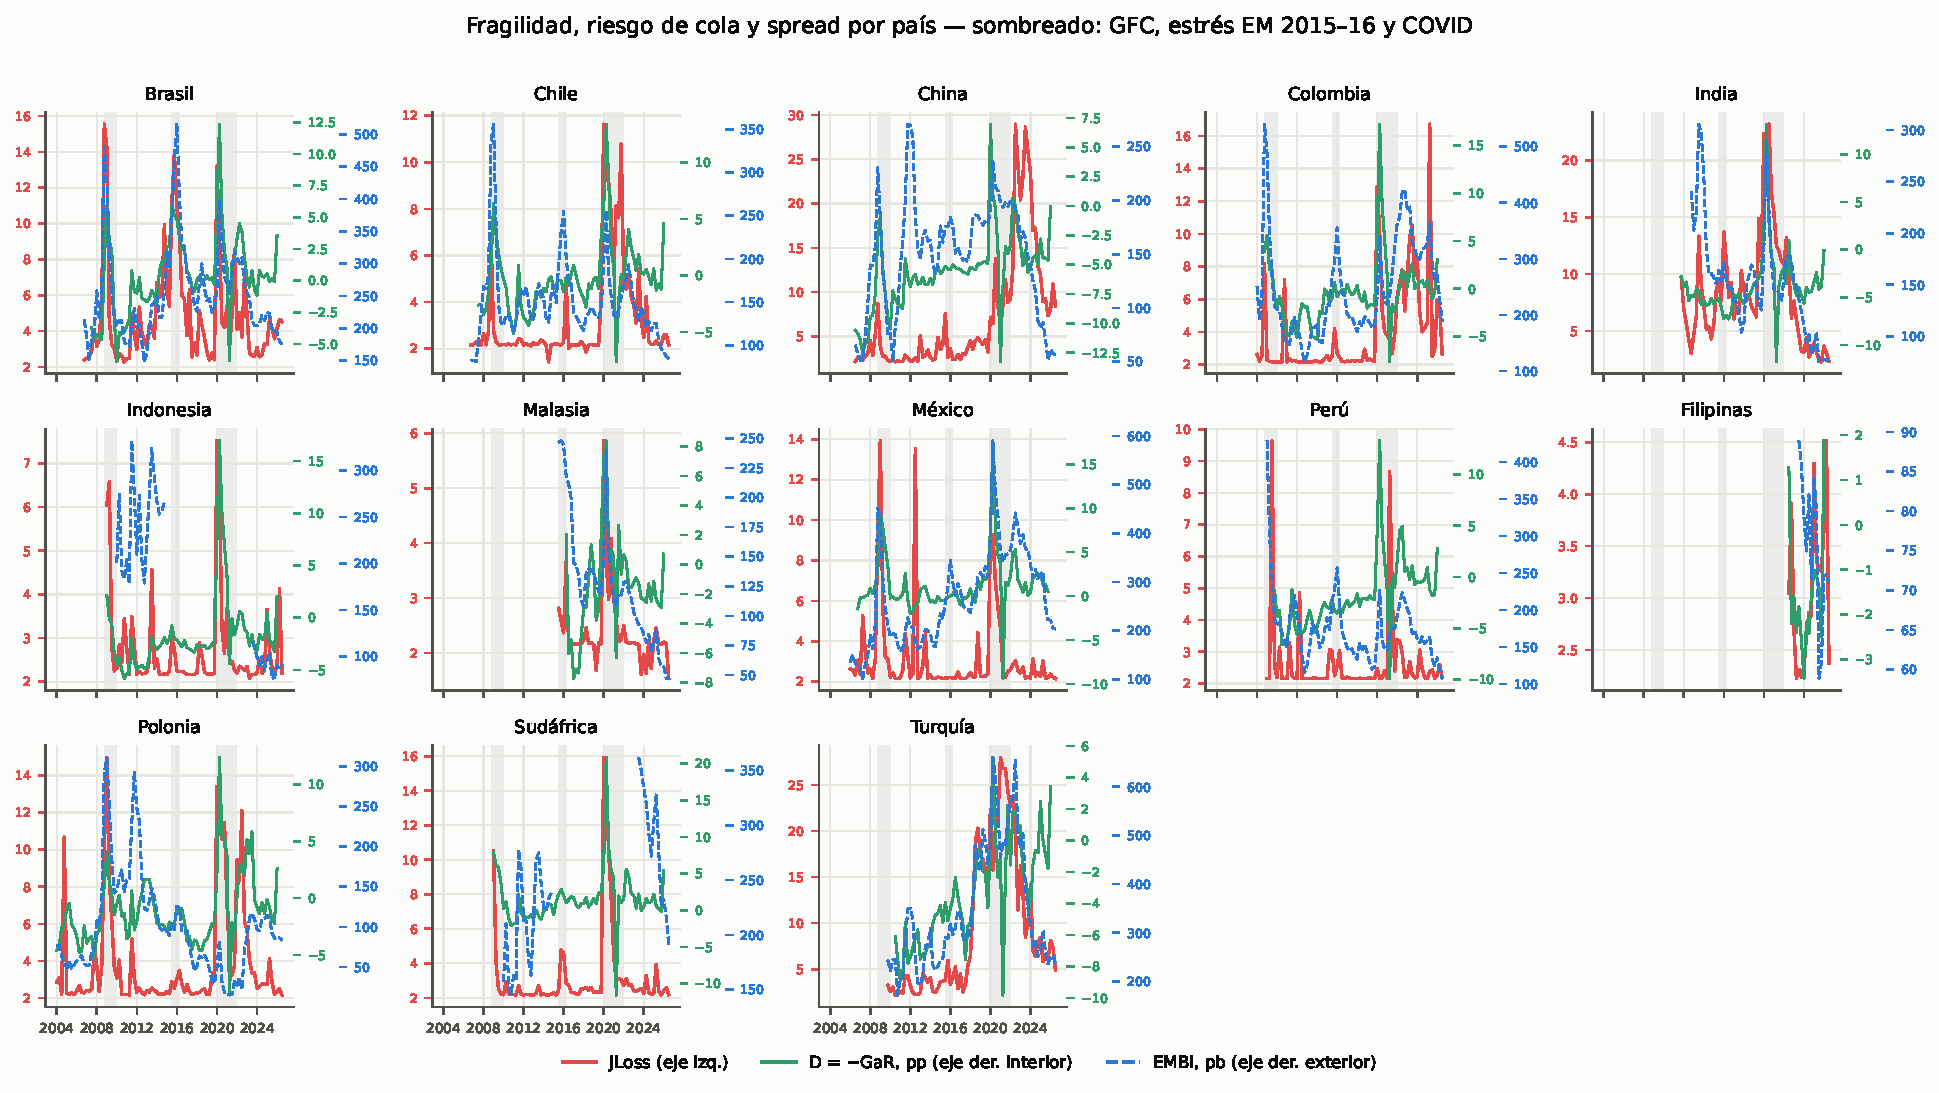
\includegraphics[width=\textwidth]{fig_series_pais_embiext.pdf}
\caption[Fragilidad, riesgo de cola y spread por país]{$JLoss$ (eje izquierdo), $D=-GaR$ (eje derecho interior) y EMBI (eje derecho exterior) por país. Sombreado: crisis financiera global (2008Q4--2009Q4), estrés emergente (2015Q3--2016Q1) y pandemia (2020Q1--2021Q4).}
\label{fig:series}
\end{figure}

La Figura~\ref{fig:comovimiento} agrega las tres series por la mediana transversal de cada trimestre, estandarizadas. $\ln JLoss_{t-1}$ y $D_{t-1}$ se mueven juntos con fuerza (correlación de 0,64 entre medianas), y cada una correlaciona 0,31 con $\ln$ EMBI. La Figura~\ref{fig:comovpais} repite el ejercicio dentro de cada país: el co-movimiento es nítido en los episodios de estrés y débil en los períodos normales.

\begin{figure}[htbp]
\centering
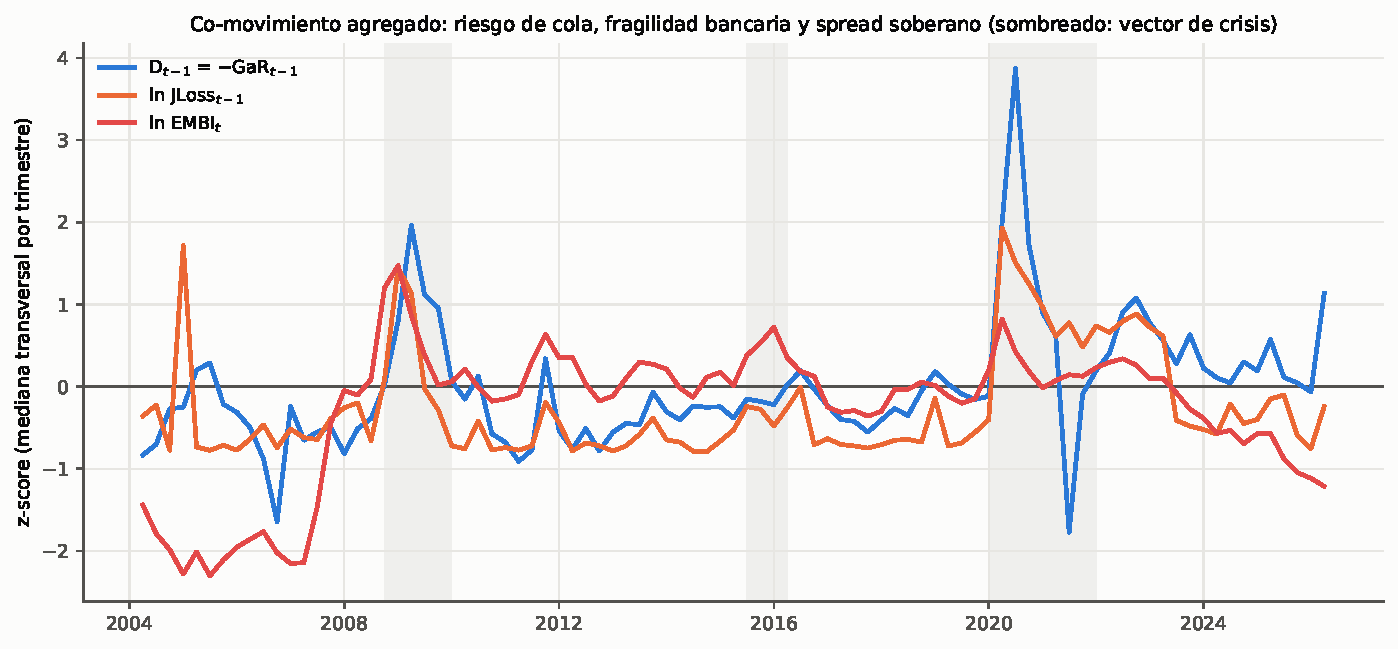
\includegraphics[width=0.9\textwidth]{fig_comovimiento_embiext.pdf}
\caption[Co-movimiento agregado]{Co-movimiento de $D_{t-1}$, $\ln JLoss_{t-1}$ y $\ln$ EMBI, estandarizados y agregados por la mediana transversal de cada trimestre. Sombreado: vector de crisis.}
\label{fig:comovimiento}
\end{figure}

\begin{figure}[htbp]
\centering
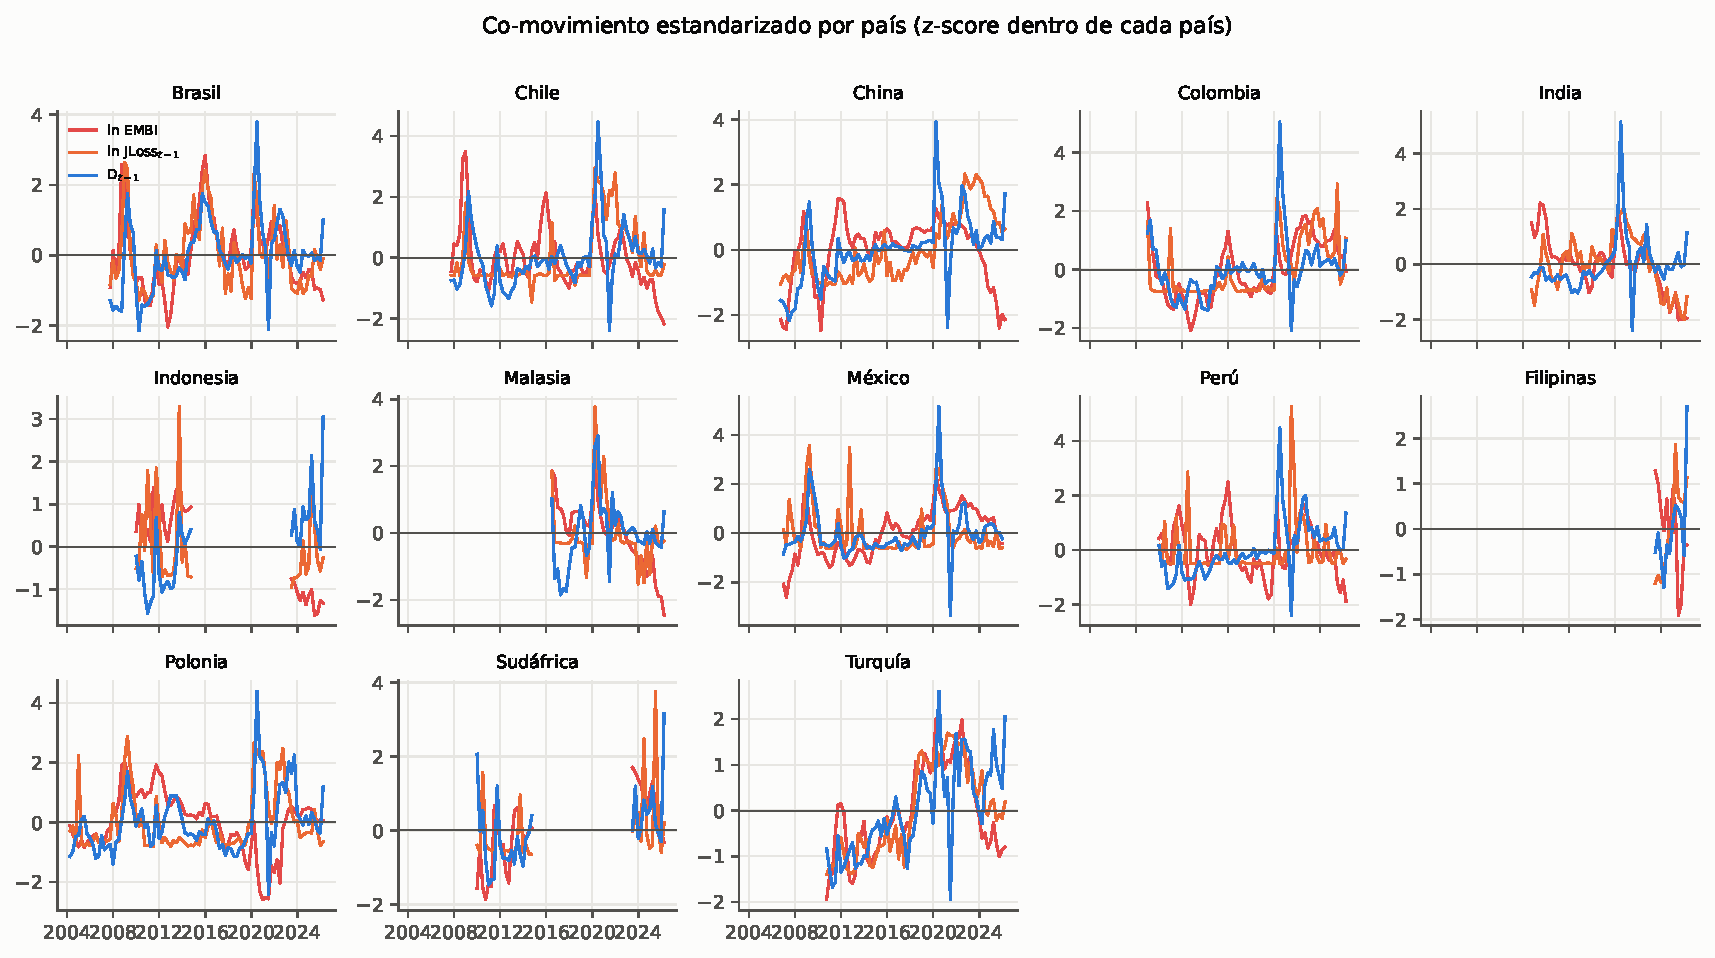
\includegraphics[width=\textwidth]{fig_comov_pais_embiext.pdf}
\caption[Co-movimiento por país]{Co-movimiento estandarizado por país ($z$-score dentro de cada país). Las líneas se cortan en los trimestres sin dato.}
\label{fig:comovpais}
\end{figure}

Por último, la Figura~\ref{fig:skewt} muestra qué mide el $GaR$ con la densidad condicional del crecimiento chileno en un trimestre benigno (2025Q3) y en el de mayor estrés (2020Q2). En el segundo, la distribución se desplaza y su cuantil 5\% cae a $-13{,}4$ puntos porcentuales.

\begin{figure}[htbp]
\centering
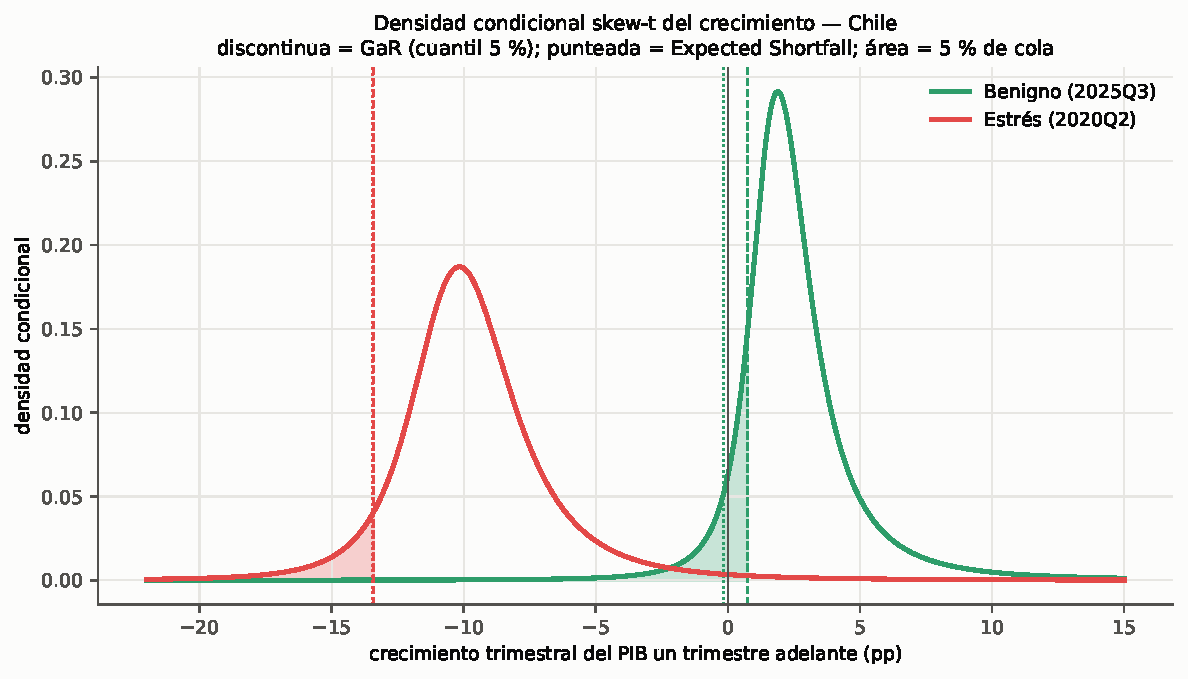
\includegraphics[width=0.85\textwidth]{fig_skewt_chile_embiext.pdf}
\caption[Densidad condicional del crecimiento]{Densidad condicional \textit{skew-t} del crecimiento de Chile en un trimestre benigno y en el de mayor estrés. Línea discontinua: $GaR$ (cuantil 5\%); punteada: \textit{Expected Shortfall}; área: 5\% de cola.}
\label{fig:skewt}
\end{figure}
